\documentclass[border=6pt]{standalone}
\usepackage{tikz}
\usepackage{amsmath}
\usetikzlibrary{positioning,arrows.meta,calc,fit,backgrounds,shapes.geometric,decorations.pathreplacing}
\definecolor{inkc}{HTML}{171A22}
\definecolor{mutedc}{HTML}{5B6274}
\definecolor{hairc}{HTML}{C9CEDA}
\definecolor{surfc}{HTML}{F2F4F8}
\definecolor{scalec}{HTML}{2E45A8}   % blue  = scale path
\definecolor{elemc}{HTML}{A65A18}    % ochre = element path
\definecolor{costc}{HTML}{B3261E}    % red   = the expensive operator
\definecolor{freec}{HTML}{1E6F4C}    % green = free / shift-only
% text macro for the small monospace annotations inside nodes
\newcommand{\dt}[1]{{\tiny\ttfamily\textcolor{mutedc}{#1}}}
\tikzset{
  blk/.style   ={draw=inkc,line width=.6pt,rounded corners=1.5pt,fill=white,
                 inner sep=4pt,align=center,font=\scriptsize},
  op/.style    ={blk,fill=surfc},
  mul/.style   ={blk,draw=costc,line width=1pt,fill=costc!7,text=costc},
  free/.style  ={blk,draw=freec,fill=freec!7,text=freec},
  scaleb/.style={blk,draw=scalec,fill=scalec!7,text=scalec},
  elemb/.style ={blk,draw=elemc,fill=elemc!7,text=elemc},
  dat/.style   ={font=\scriptsize\ttfamily,text=mutedc},
  lbl/.style   ={font=\scriptsize,text=mutedc,align=center},
  ttl/.style   ={font=\small\bfseries,text=inkc},
  ar/.style    ={-{Stealth[length=4pt,width=3pt]},draw=inkc,line width=.5pt},
  arS/.style   ={ar,draw=scalec},
  arE/.style   ={ar,draw=elemc},
}

\begin{document}
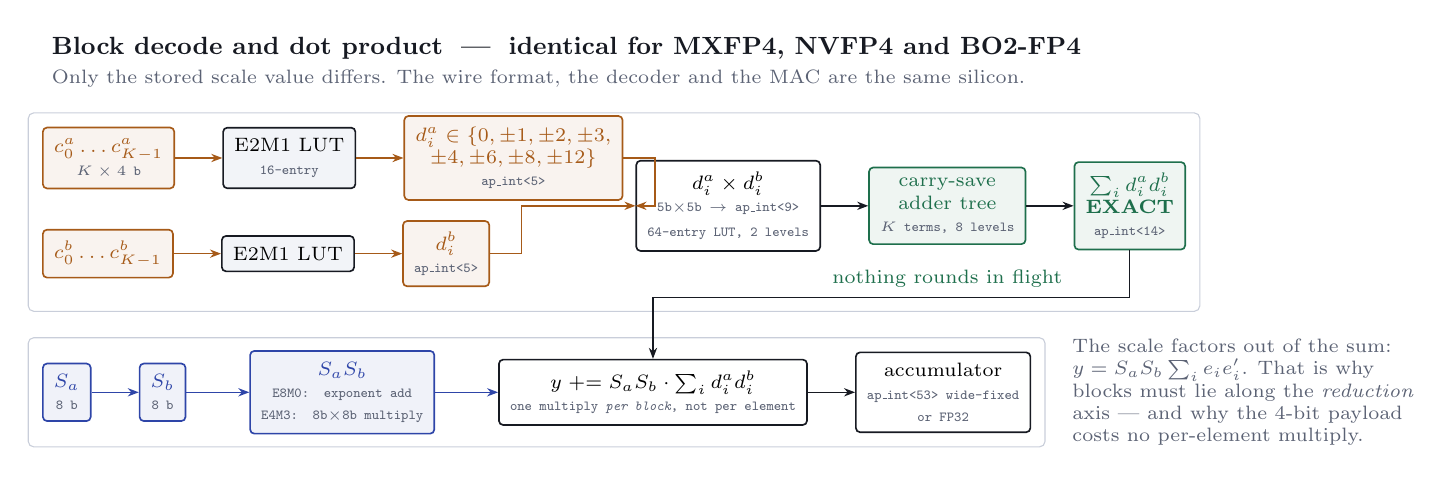
\begin{tikzpicture}[node distance=6mm]

\node[ttl] (t) {Block decode and dot product \;---\; \textbf{identical} for MXFP4, NVFP4 and BO2-FP4};
\node[lbl,below=1.5mm of t.west,anchor=north west,align=left]
  {Only the stored scale value differs. The wire format, the decoder and the MAC are the same silicon.};

% ---- operand A -----------------------------------------------------------
\node[elemb,below=10mm of t.west,anchor=north west] (ca) {$c^a_0\dots c^a_{K-1}$\\\dt{$K\times4$ b}};
\node[op,right=of ca] (lta) {E2M1 LUT\\\dt{16-entry}};
\node[elemb,right=of lta] (da) {$d^a_i \in \{0,\pm1,\pm2,\pm3,$\\$\pm4,\pm6,\pm8,\pm12\}$\\\dt{\texttt{ap\_int<5>}}};
\draw[arE](ca)--(lta); \draw[arE](lta)--(da);

\node[elemb,below=9mm of ca.west,anchor=north west] (cb) {$c^b_0\dots c^b_{K-1}$};
\node[op,right=of cb] (ltb) {E2M1 LUT};
\node[elemb,right=of ltb] (db) {$d^b_i$\\\dt{\texttt{ap\_int<5>}}};
\draw[arE](cb)--(ltb); \draw[arE](ltb)--(db);

% ---- the exact integer core ---------------------------------------------
\node[blk,right=10mm of $(da.east)!0.5!(db.east)$,yshift=0mm] (mul)
  {$d^a_i \times d^b_i$\\\dt{5b$\times$5b $\to$ \texttt{ap\_int<9>}}\\[1pt]\dt{64-entry LUT, 2 levels}};
\draw[arE](da.east)-|++(4mm,0)|-(mul.west);
\draw[arE](db.east)-|++(4mm,0)|-(mul.west);
\node[free,right=of mul] (tree) {carry-save\\adder tree\\\dt{$K$ terms, 8 levels}};
\node[free,right=of tree] (core) {$\sum_i d^a_i d^b_i$\\\textbf{EXACT}\\\dt{\texttt{ap\_int<14>}}};
\draw[ar](mul)--(tree); \draw[ar](tree)--(core);
\node[lbl,below=2mm of tree.south,align=center,text=freec,font=\scriptsize] (nr)
  {nothing rounds in flight};

% ---- the scale path ------------------------------------------------------
\node[scaleb,below=26mm of ca.west,anchor=north west] (sa) {$S_a$\\\dt{8 b}};
\node[scaleb,right=of sa] (sb) {$S_b$\\\dt{8 b}};
\node[scaleb,right=8mm of sb] (sp) {$S_a S_b$\\\dt{E8M0: exponent \textbf{add}}\\\dt{E4M3: 8b$\times$8b multiply}};
\draw[arS](sa)--(sb); \draw[arS](sb)--(sp);

\node[blk,right=8mm of sp] (fin) {$y \;{+}{=}\; S_aS_b \cdot \textstyle\sum_i d^a_id^b_i$\\\dt{one multiply \emph{per block}, not per element}};
\draw[arS](sp)--(fin);
\draw[ar](core.south)--++(0,-6mm)-|(fin.north);
\node[blk,right=of fin] (acc) {accumulator\\\dt{\texttt{ap\_int<53>} wide-fixed}\\\dt{or FP32}};
\draw[ar](fin)--(acc);

\node[lbl,right=4mm of acc,align=left]
  {The scale factors out of the sum:\\
   $y=S_aS_b\sum_i e_ie'_i$. That is why\\
   blocks must lie along the \emph{reduction}\\
   axis --- and why the 4-bit payload\\
   costs no per-element multiply.};

\begin{scope}[on background layer]
  \node[fit=(ca)(db)(core)(nr),draw=hairc,rounded corners=2pt,inner sep=5pt,label={[lbl,anchor=north west]north west:\;}]{};
  \node[fit=(sa)(acc),draw=hairc,rounded corners=2pt,inner sep=5pt]{};
\end{scope}
\end{tikzpicture}
\end{document}
